\chapter{Stimmhaftigkeit}

\section{Stichworte zur Vorlesung \em{Aerodynamische Prozesse und Phonation}}

ingressiv, egressiv, Ejektiv, Implosiv, Klicklaut, Bernoulli-Prinzip, Voice onset time (VOT), supra- und subglottaler Luftdruck\dots $\rightarrow$ {\tt L6\underline{\ }Phonation.pdf}

\begin{figure}[htbp]
\begin{center}
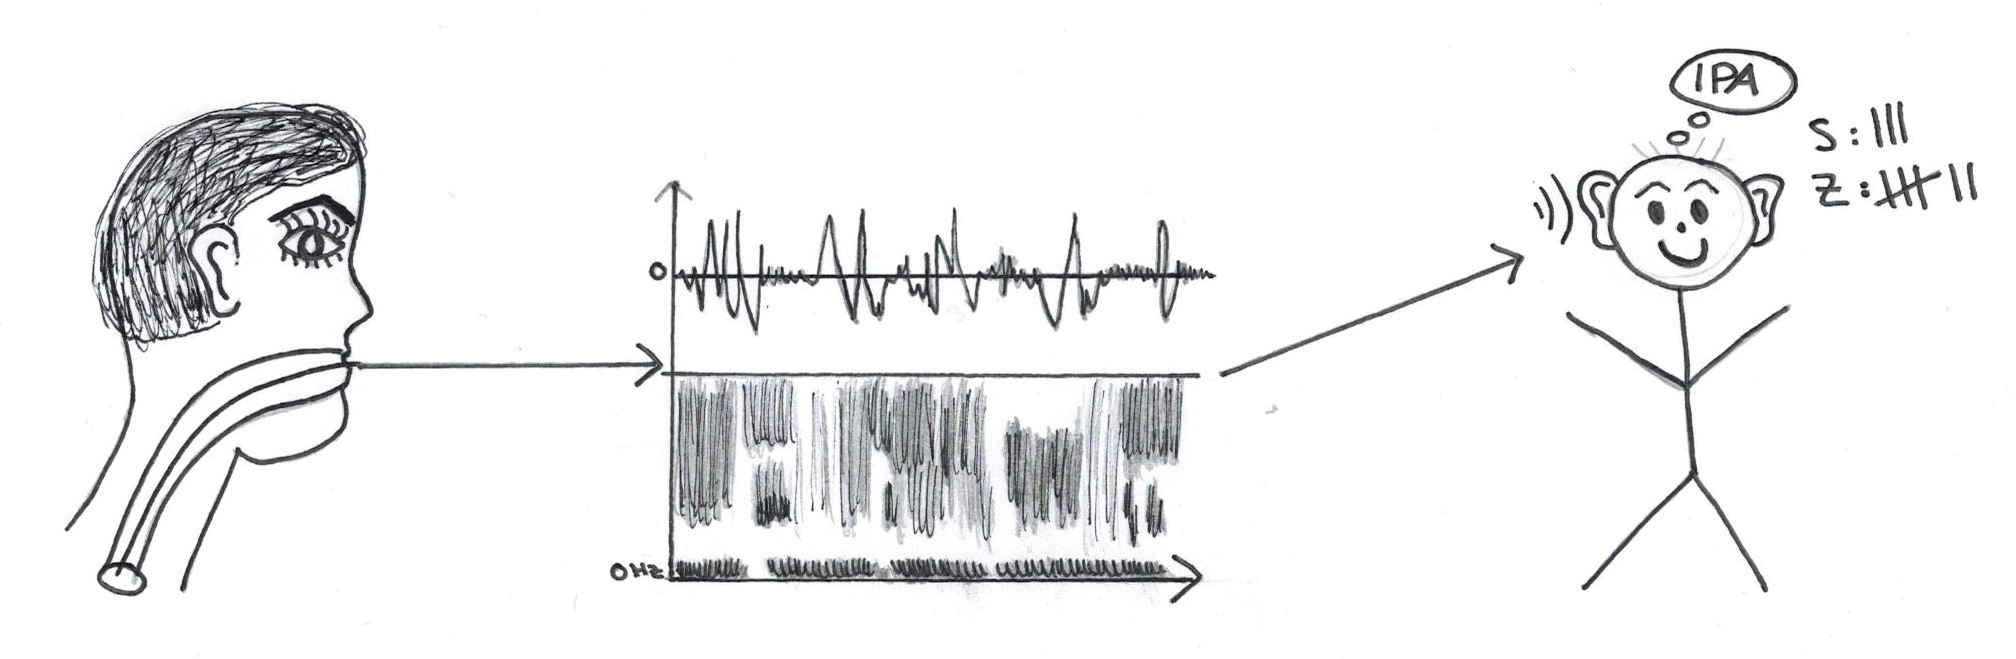
\includegraphics[width=\textwidth]{grafiken/stimmhaftigkeit/stimmhaftigkeit.jpg}
\label{t4}
\end{center}
\end{figure}


\newpage
\section{Übungen}

1.	Suchen Sie in Ihren Aufnahmen nach Segmenten, die sie mit einem Symbol etikettiert haben, das Stimmhaftigkeit signalisiert (z.\,B. b, a, n). In welchen Fällen handelt es sich um phonetisch stimmhafte Laute, in welchen nicht?
\vspace{4cm}

2.	Gibt es eine Systematik zwischen stimmhaften Etiketten und fehlender phonetischer Stimmhaftigkeit?
\vspace{4cm}
